\documentclass[a4paper, 12pt]{article}
\usepackage[top=3cm, bottom=2cm, left=2cm, right=3cm]{geometry}
\usepackage[utf8]{inputenc}
\usepackage{amsmath, amsfonts, amssymb}
\usepackage{graphicx, xcolor}
\usepackage{tikz}
\usepackage{subfig}
\usetikzlibrary{arrows.meta}
\usetikzlibrary{calc}
\usepackage{scalerel, pict2e, tkz-euclide}
\usetikzlibrary{calc, patterns, arrows.meta,shadows,external}

\usepackage{pgfplots}
\usepackage{cancel}
\usepackage{enumitem}
\pgfplotsset{compat=newest}
\usepgfplotslibrary{statistics,fillbetween}
\usepackage{indentfirst}

\begin{document}
	\author{Leandro Júnior Cândido de Oliveira}
	\title{Notebook Calculus}
	
	\maketitle
	
	\section{Limits and Derivatives}
	
	\subsection{The Tangent and Velocity Problems}
	
	\subsubsection{The Tangent Problem}
	
	EXAMPLE 1: Find a equation for the tangent line to the parabola $y=x^2$ at the point $P=(1,1)$.
	
	\textit{My solution}:
	
	\begin{figure}[htp]
		\centering
		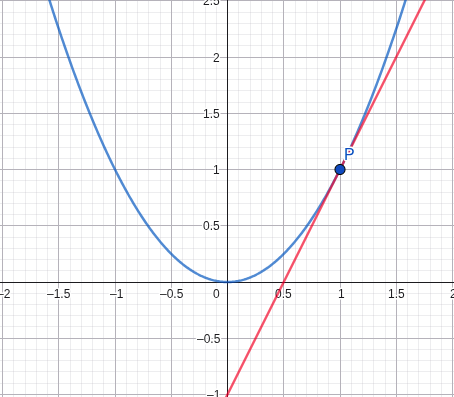
\includegraphics[width=0.5\linewidth]{Captura de tela de 2026-05-03 19-40-17.png}
	\end{figure}
	
	For to find a equation for a line we need two points in the line. For the problem the only point of the line is $P$. My idea is evaluate a second point in the tangent line that is in the parabola. For a good precision will select the point $(0.1,f(0.1))$:
	

	slop: \[m=\frac{1-f(0.1)}{1-0.1}=1.9\]
	
	coefficient $b$:\[b=1-1\cdot 1.9=0.9\]
	
	Therefore, the equation for the tangent line is approx: \[g(x)=1.9x-0.9\]  	
	
	\subsubsection{The Velocity Problem}
	
	EXAMPLE 3: Suppose that a ball is dropped from the upper observation deck of the CN Tower in Toronto, 450 m above the ground. Find the velocity of the ball after 5 seconds.
	
	\textit{My solution:}
	
	  
	
\end{document}